\newcommand{\psd}[1]{{\small\sffamily{\color{blue!60}#1}}}


The problem of interest is a single Dirichlet condition problem of
soildynamics in 2D. For this problem we use Newmark-\(\beta\) time
discretization. Additionally postrocessing is demanded for displacement,
acceleration, and velocity (\(u,a,v\)).

\begin{lstlisting}[style=BashInputStyle]
PSD_PreProcess -dimension 2 -problem soildynamics -dirichletconditions 1 -timediscretization newmark_beta \
-postprocess uav
\end{lstlisting}

Once the step above has been performed, we solve the problem using four
MPI processes, with the given mesh file \psd{soil.msh}.

\begin{lstlisting}[style=BashInputStyle]
PSD_Solve -np 4 Main.edp -mesh ./../Meshes/2D/soil.msh -v 0
\end{lstlisting}

\begin{figure}[h!]
\centering
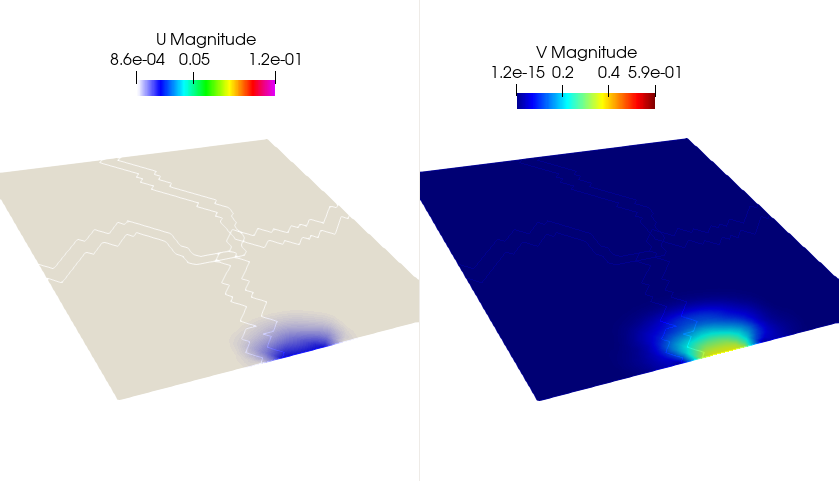
\includegraphics[width=0.4\textwidth]{./Images/sd-u0.png}
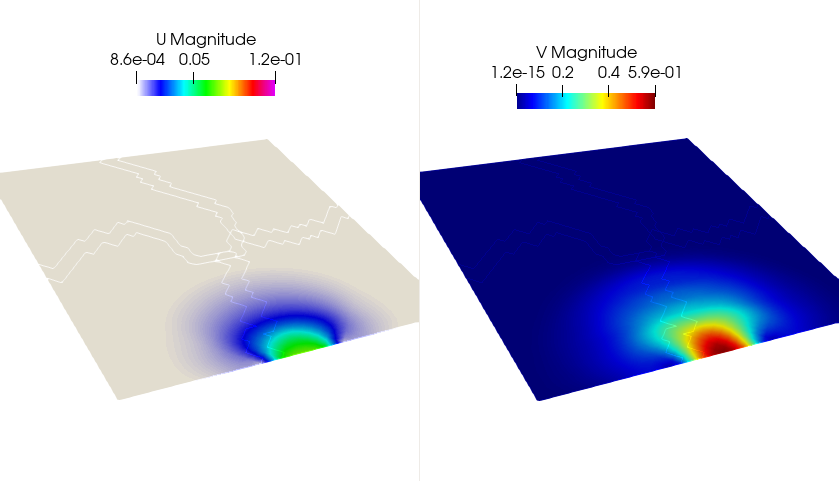
\includegraphics[width=0.4\textwidth]{./Images/sd-u1.png}\\
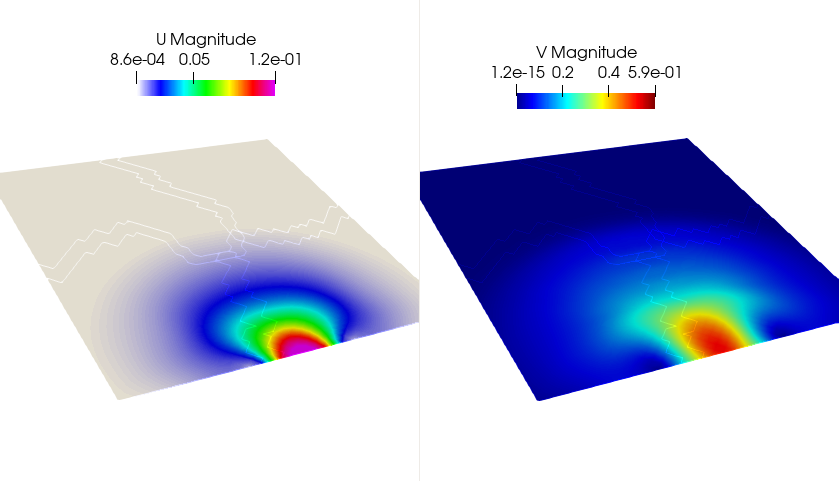
\includegraphics[width=0.4\textwidth]{./Images/sd-u2.png}
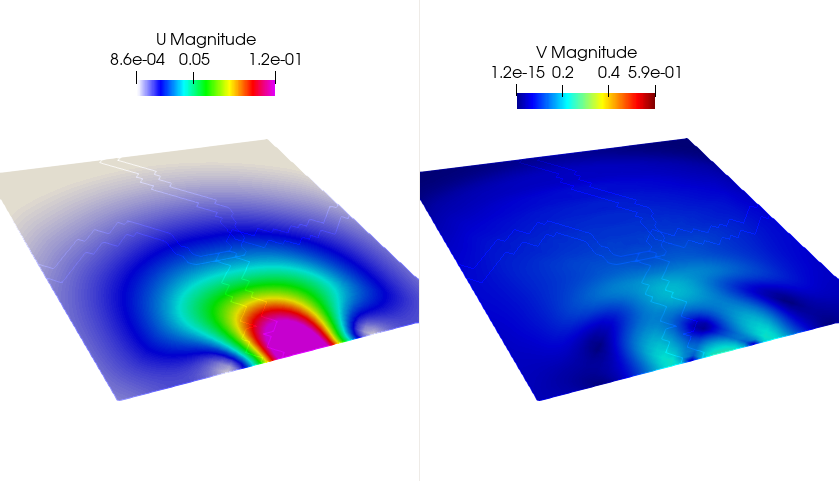
\includegraphics[width=0.4\textwidth]{./Images/sd-u3.png}\\
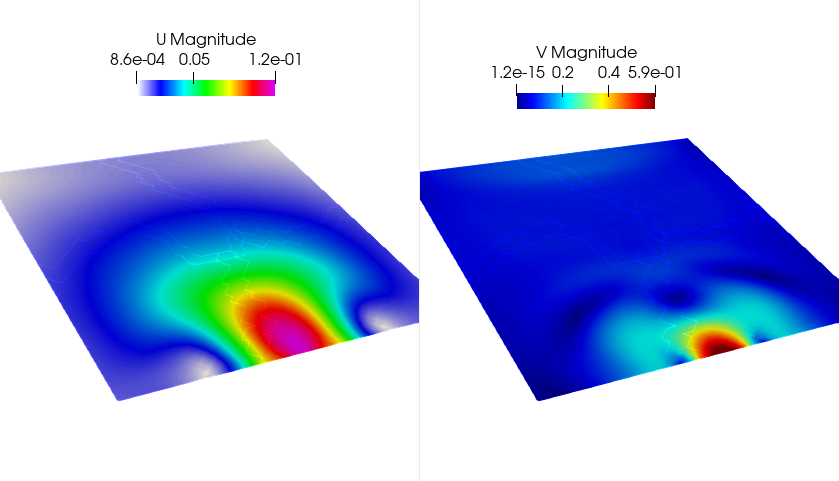
\includegraphics[width=0.4\textwidth]{./Images/sd-u4.png}
\caption{Finite element displacement and velocity fields visualized for the 2D problem with ParaView at different timesteps. \label{bar-sd}}
\end{figure}

Using ParaView for postprocessing the results that are provided in the
\psd{VTUs...} folder, results such as those shown in
figure\textasciitilde{}\ref{bar-sd} can be extracted.
